% !TeX spellcheck = en_US	


\documentclass[10pt,journal,compsoc]{IEEEtran}
\usepackage{graphicx}
\usepackage[ruled, linesnumbered]{algorithm2e}
\usepackage{url}
\usepackage{epstopdf}
\usepackage{indentfirst}
\usepackage[tight,footnotesize]{subfigure}
\usepackage{amsmath}
\usepackage{amssymb}
\usepackage{multirow}
\usepackage{color}
\usepackage{enumerate}

\newtheorem{Formula}{Formula}
\newtheorem{Lemma}{Lemma}
\newtheorem{Corollary}{Corollary}
\newtheorem{Property}{Property}
\newtheorem{Rule}{Rule}

% *** CITATION PACKAGES ***
\ifCLASSOPTIONcompsoc
\usepackage[nocompress]{cite}
\else
\usepackage{cite}
\fi


\begin{document}

\appendices
\section{Overview on the Induction Phase} \label{sec:appendix}

Notice that ${\sf suf}(i) < {\sf suf}(j)$ if (1) $x[i] < x[j]$ or (2) $x[i] = x[j]$ and ${\sf suf}(i + 1) < {\sf suf}(j + 1)$; otherwise, ${\sf suf}(i) > {\sf suf}(j)$. This observation is utilized by the IS algorithms to sort suffixes as follows:

\begin{enumerate}[S1]
	\item 
	Clear S-type sub-buckets in $sa$. Scan $sa^*$ leftward and insert each element into the current rightmost empty position in the corresponding S-type sub-bucket.
	
	\item 
	Clear L-type sub-buckets in $sa$ and insert $n - 1$ into the leftmost position in ${\sf sa\_bkt_L}(x[n - 1])$. Scan $sa$ rightward with $i$ increasing from $0$ to $n - 1$. For each scanned non-empty $sa[i]$ with $t[sa[i] - 1] = 0$, insert $sa[i] - 1$ into the current leftmost empty position in ${\sf sa\_bkt_L}(x[sa[i] - 1])$.
	
	\item
	Clear S-type sub-buckets in $sa$. Scan $sa$ leftward with $i$ decreasing from $n - 1$ to $0$. For each scanned non-empty $sa[i]$ with $t[sa[i] - 1] = 1$, insert $sa[i] - 1$ into the current rightmost empty position in ${\sf sa\_bkt_S}(x[sa[i] - 1])$.
	
\end{enumerate}

In brief, given $sa^*$, S1 inserts all the S*-type suffixes into $sa$ in their lexical order. Then, S2-S3 induce the order of L- and S-type suffixes from those already sorted in $sa$, respectively, where the relative order of two suffixes induced into the same sub-bucket matches their insertion order according to the rule stated above. To be more specific, we show in Fig.~\ref{fig:example2} a running example of the induction phase.

As depicted, the input string $x$ contains 6 S*-type suffixes sorted in line 3. When finished inserting the S*-type suffixes in lines 5-6, we first find the head of each L-type sub-bucket (marked by the symbol $\wedge$) and insert ${\sf suf}(13)$ into $sa$. Notice that ${\sf suf}(13)$ consists of only one character, it must be the smallest L-type suffixes starting with $1$. Thus, we put ${\sf suf}(13)$ into the leftmost position in ${\sf sa\_bkt_L}(1)$ in line 8. Then, we scan $sa$ from left to right for inducing the order of all the L-type suffixes. In lines 10-11, when visiting $sa[0] = 13$ (marked by the symbol $@$), we check the type array $t$ to find $x[12] = 2$ is L-type and hence insert ${\sf suf}(12)$ into the current leftmost empty position in ${\sf sa\_bkt_L}(2)$. Similarly, in lines 12-13, we visit the next scanned item $sa[1] = 11$ and see that $t[10] = 0$, thus we place ${\sf suf}(10)$ into the current head of ${\sf sa\_bkt_L}(3)$. Following this way, we get all the L-type suffixes sorted in $sa$. After that, we first find the end of each S-type sub-bucket in lines 25-26 and scan $sa$ leftward for inducing the order of all the S-type suffixes in lines 27-40. When visiting $sa[13] = 2$, we see $x[1]$ is S-type and thus put ${\sf suf}(1)$ into the current rightmost empty position in ${\sf sa\_bkt_S}(1)$. Then, at $sa[12] = 8$, we see $x[7] = 1$ is S-type and thus put ${\sf suf}(7)$ into the current rightmost empty position in ${\sf sa\_bkt_S}(1)$. To repeat scanning $sa$ in this way, we get all the S-type suffixes sorted in $sa$. 

The work in~\cite{Fischer11} describes how to compute the LCP array during the execution of S2-S3. Given two suffixes placed at the neighboring positions in $sa$, their LCP-value can be computed according to one of the following two cases in respect to whether or not they are inserted into the same sub-bucket: if yes, then their LCP-value is one greater than that of the two suffixes from which inducing them; otherwise, their LCP-value equals to zero. In this way, we can determine $lcp[i]$ immediately after the computation of $sa[i]$. The problem here is how to obtain the LCP-values of these inducing suffixes starting at the next positions in $x$, which is modeled as a range minimum query in~\cite{Fischer11} and can be answered within amortized $\mathcal{O}(1)$ time. For example, when scanning $sa[0]$ and $sa[5]$ in lines 10-11 and 20-21 of Fig.~\ref{fig:example2}, ${\sf suf}(12)$ and ${\sf suf}(6)$ are sequentially induced into the neighboring positions in ${\sf sa\_bkt_L(2)}$. In the meantime, if we keep recording the minimum over $lcp(0, 5]$, then we can obtain the LCP-value of the inducing suffixes ${\sf suf}(13)$ and ${\sf suf}(7)$ when putting the induced suffix ${\sf suf}(6)$ into $sa$.

\begin{figure}
	\centering
	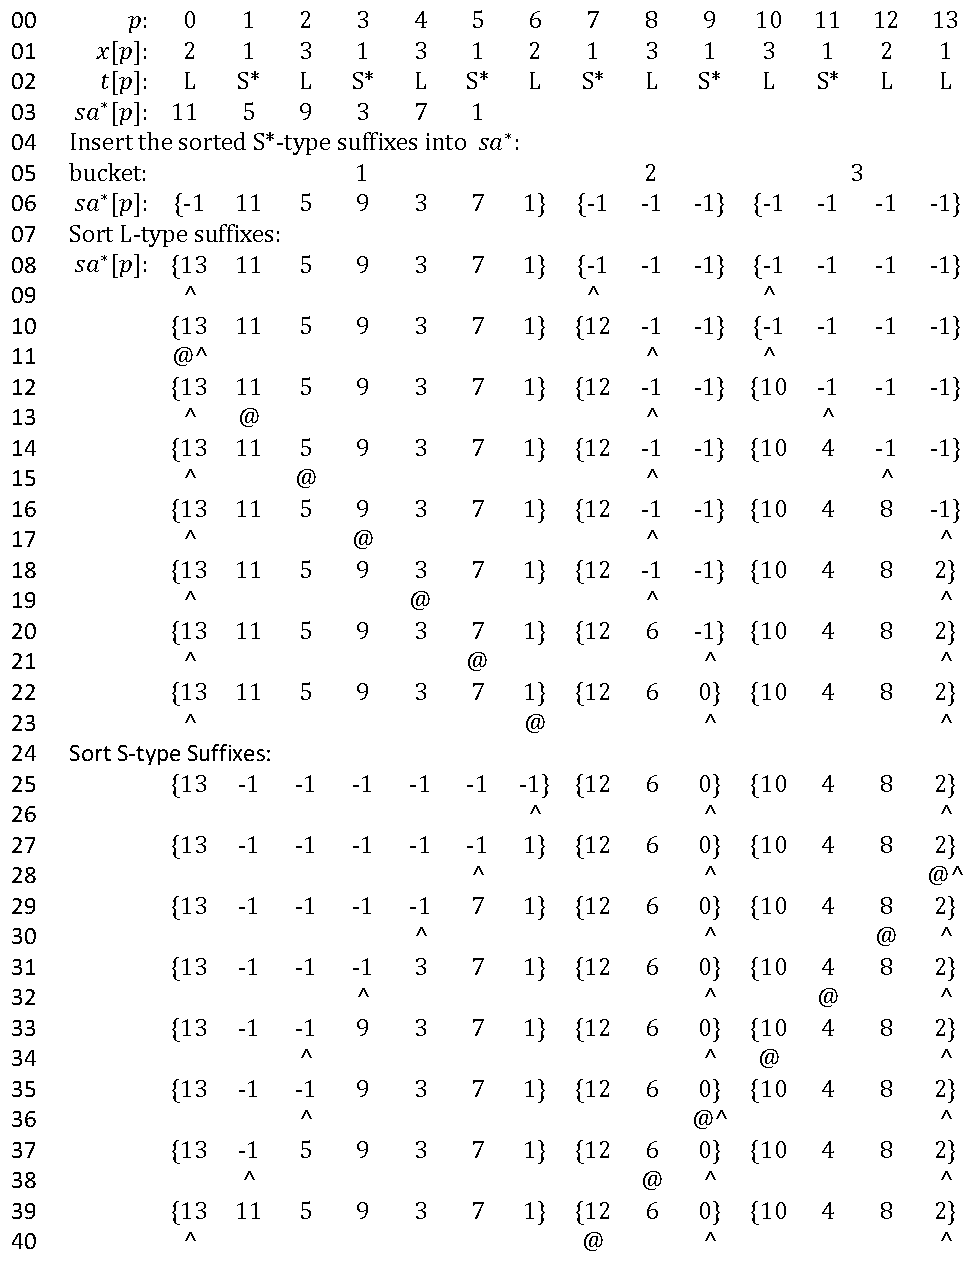
\includegraphics[width = 0.9\columnwidth]{example2}

	\caption{An Example for inducing the suffix and LCP arrays. \label{fig:example2}}	
\end{figure}
 
	
\end{document}






























